\section{Spektren}

\subsection{Versuch 4}

\begin{figure}[h]
 \centering
 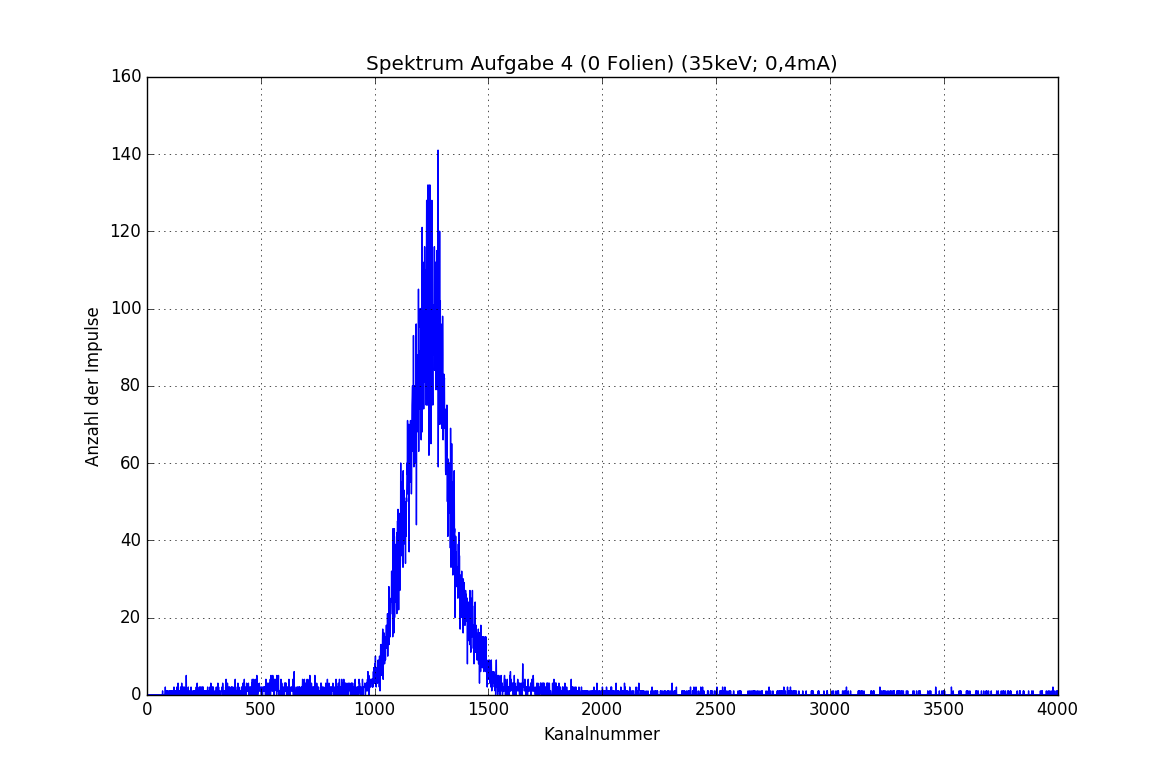
\includegraphics[scale=0.5]{./fig/a4_spec0.png}
 \caption{Spektrum für Versuch 4 (0 Folien)}
 \label{fig:spek40}
\end{figure}

\begin{figure}[h]
 \centering
 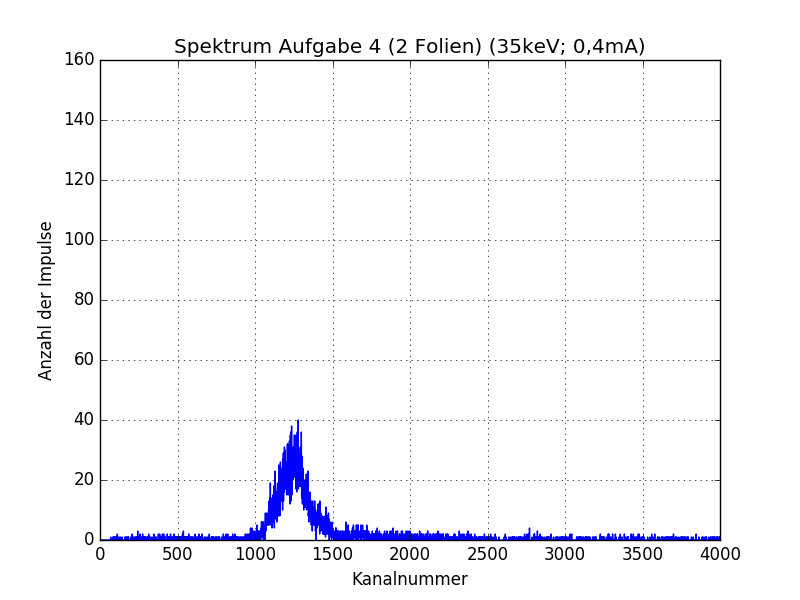
\includegraphics[scale=0.7]{./fig/a4_spec2.png}
 \caption{Spektrum für Versuch 4 (2 Folien)}
 \label{fig:spek42}
\end{figure}

\begin{figure}[h]
 \centering
 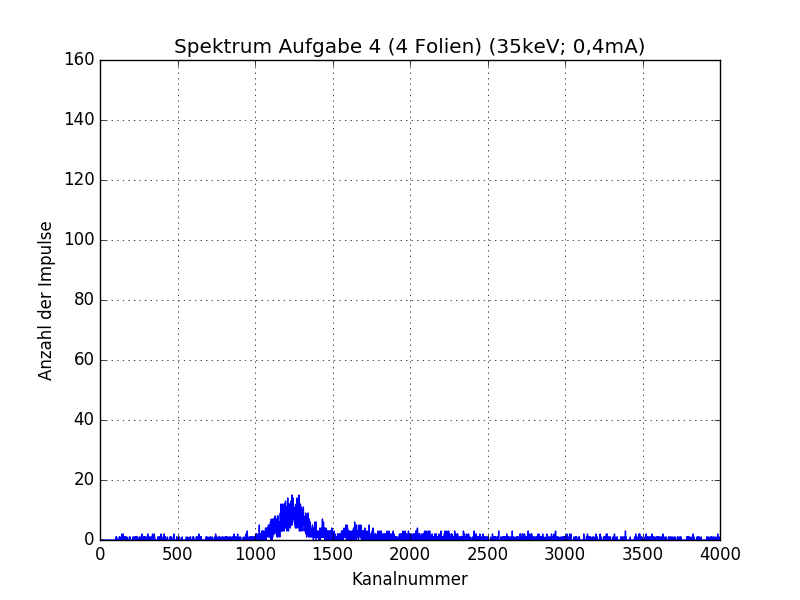
\includegraphics[scale=0.7]{./fig/a4_spec4.png}
 \caption{Spektrum für Versuch 4 (4 Folien)}
 \label{fig:spek44}
\end{figure}

\begin{figure}[h]
 \centering
 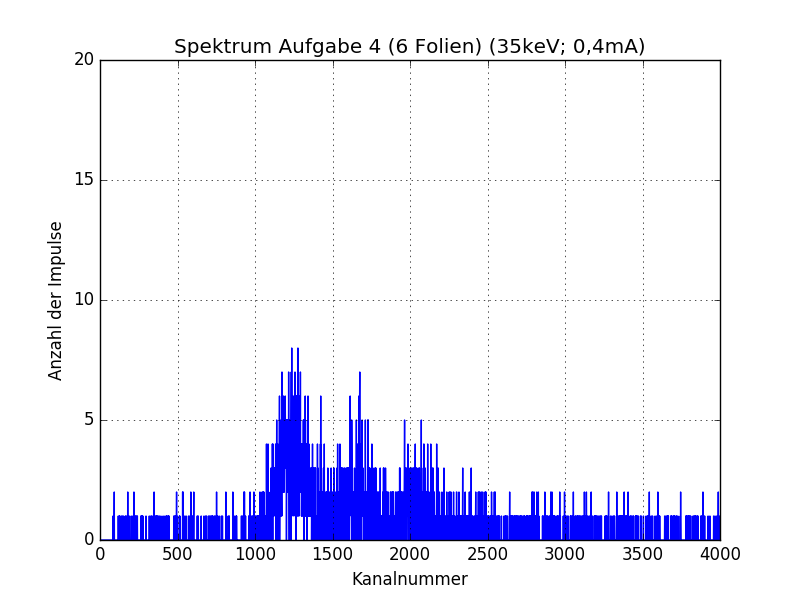
\includegraphics[scale=0.7]{./fig/a4_spec6.png}
 \caption{Spektrum für Versuch 4 (6 Folien)}
 \label{fig:spek46}
\end{figure}

\subsection{Versuch 5}

\begin{figure}[h]
 \centering
 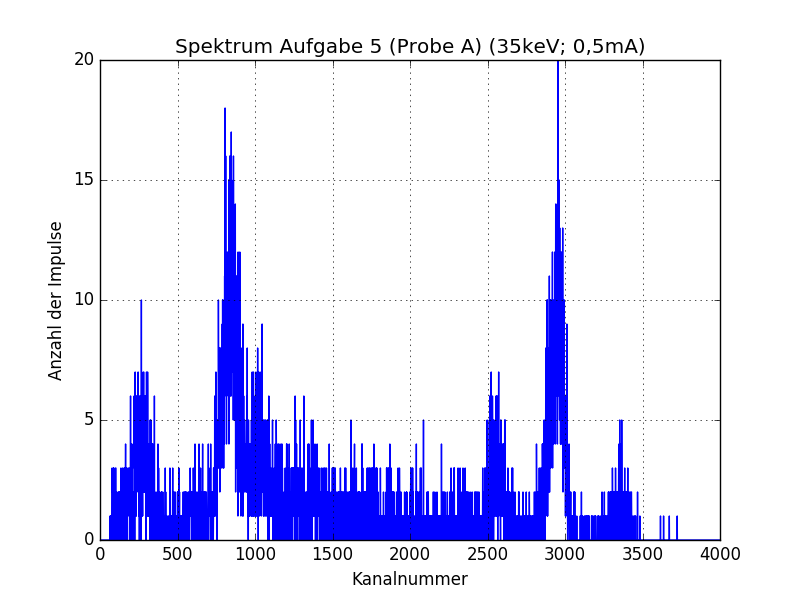
\includegraphics[scale=0.7]{./fig/a5_speca.png}
 \caption{Spektrum für Versuch 5 (Probe A)}
 \label{fig:spek4a}
\end{figure}

\begin{figure}[h]
 \centering
 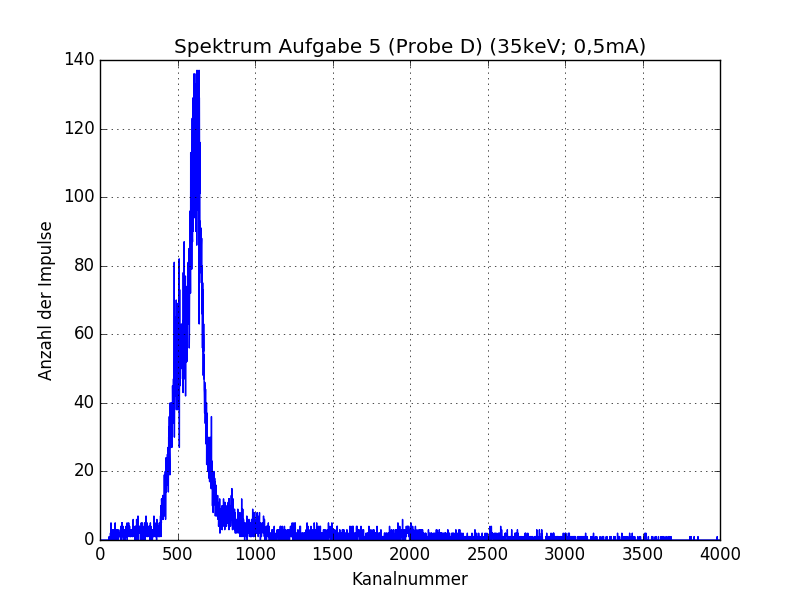
\includegraphics[scale=0.7]{./fig/a5_specd.png}
 \caption{Spektrum für Versuch 5 (Probe D)}
 \label{fig:spek4d}
\end{figure}

\begin{figure}[h]
 \centering
 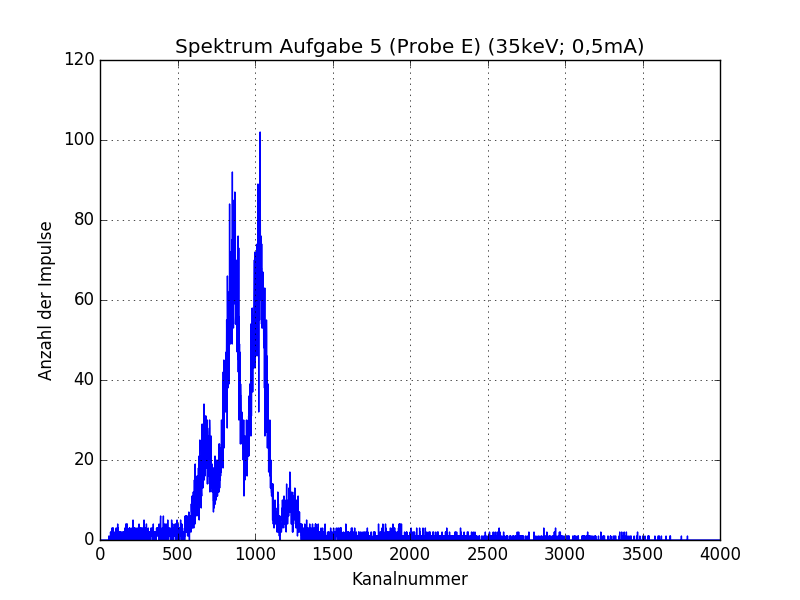
\includegraphics[scale=0.7]{./fig/a5_spece.png}
 \caption{Spektrum für Versuch 5 (Probe E)}
 \label{fig:spek4e}
\end{figure}

\begin{figure}[h]
 \centering
 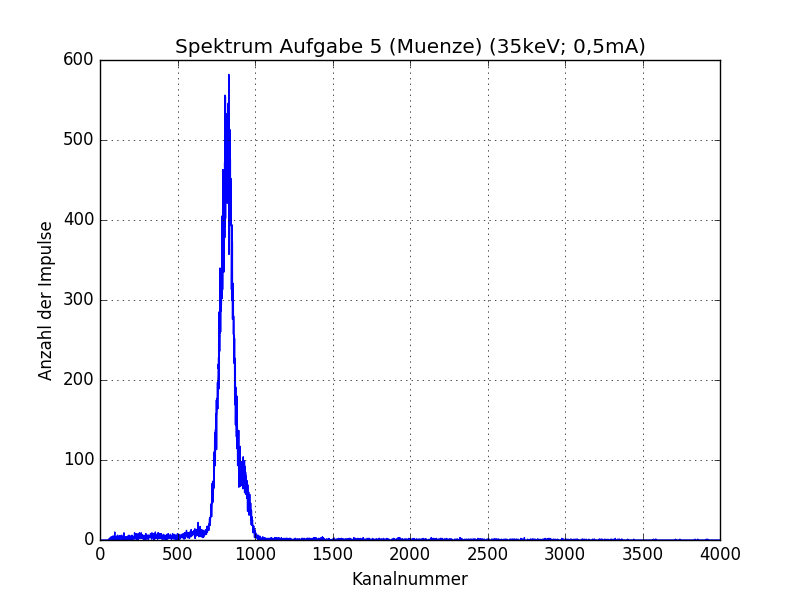
\includegraphics[scale=0.7]{./fig/a5_specm.png}
 \caption{Spektrum für Versuch 5 (Münze)}
 \label{fig:spek4m}
\end{figure}


